\documentclass[10pt,letterpaper]{article}
\usepackage[utf8]{inputenc}
\usepackage{amsmath}
\usepackage{amsfonts}
\usepackage{amssymb}
\usepackage{graphicx}
\usepackage{hyperref}
\usepackage{siunitx}
\DeclareSIUnit{\torr}{torr}
\sisetup{retain-unity-mantissa = false}
\sisetup{separate-uncertainty=true}
\usepackage{booktabs}
\usepackage{ulem}
\usepackage{rotating}

\author{W. Schreyer}
\title{Fall run 2019 -- analysis report}
\begin{document}

\maketitle

\tableofcontents

\section{Introduction}

This document describes several analyses of the data taken during the 2019 run of the UCN source at TRIUMF, covering measurements of
\begin{itemize}
\item transmission through guide components,
\item storage lifetime in the source, and
\item storage lifetime in guide components.
\end{itemize}

All these experiments are performed in cycles. Each cycle contains several periods, typically starting with an irradiation period, during which the target is irradiated with protons and ultracold neutrons are produced. This can be followed by up to 9 more periods, like storage or detection periods. For each period, up to 8 UCN components like valves or spin flippers can be to set different states. The last (11th) period covers the time until the next irradiation and cycle starts.

Cycles with different period durations and valve settings can be grouped in supercycles, which can be repeated several times. Cycles of one experiment can be spread over several Midas runs.

Two UCN detectors were used throughout the run. A Li6 detector, detecting scintillation light of UCN captured in $^6$Li-enriched glass, and a He3 detector, detecting gas discharges due to UCN captured by $^3$He. Experiments can use either detector alone or both at the same time.


\section{Preparation of raw detector data}

\subsection{Trigger thresholds}

The Li6 detector uses two values to determine if a detected event was actually caused by a UCN: ``PSD'' based on the pulse shape of the event and $Q_\mathrm{long}$, the charge collected during a \SI{200}{\nano\second} window after the event trigger. An event is considered a UCN if
\begin{equation}
\mathrm{PSD} > 0.3
\end{equation}
and
\begin{equation}
Q_\mathrm{long} > 2000.
\end{equation}

The He3 detector considers an event to be a UCN if the charge collected after the event trigger
\begin{equation}
Q_\mathrm{short} > 300.
\end{equation}

%\subsection{Excluded events}

%In some experiments with high gas pressures in the UCN guide we saw the rate in the Li6 detector spike when a valve moved. Affected runs identified so far are 1153 to 1160 and 1203 to 1205. These were all part of measurements at high He-II temperatures and high vapor pressures, or measurements with high nitrogen pressures injected into the UCN guide. In these runs, the events in the Li6 detector within the first second of each period were binned into \SI{1}{\milli\second}-wide bins and all events in bins that had more than three entries were discarded. In total, about \num{70000} events were discarded from 72 cycles this way.


\section{Transmission measurements}

Transmission measurements are experiments with three periods per cycle. An irradiation period, $t_i$, where UCN are produced while the valve IV2 downstream of the He3 detector is closed. A pre-storage period $t_p$, where the irradiation is stopped and the source valve IV1 is closed, storing UCN between IV1 and IV2 while monitoring the rate in the He3 detector connected to this volume. And a counting period, $t_c$, where the UCN valve is opened and UCN transmitted through components downstream of the valve are detected in the Li6 detector.

The UCN counted in the He3 detector during the pre-storage period give a measure or how many UCN are available for transmission to the Li6 detector once IV2 opens. Hence, the ratio
\begin{equation}
R_p = \frac{N^\mathrm{Li6}_c}{N^\mathrm{He3}_p}
\end{equation}
of UCN seen in the Li6 detector $N^\mathrm{Li6}_c$ to the UCN seen in the He3 detector $N^\mathrm{He3}_p$ is a measure of how well UCN can be transmitted through the guides between the valve and the Li6 detector.

A background rate $b^\mathrm{Li6}$ estimated during the pre-storage periods is subtracted from the number of events counted in the Li6 detector during counting $C^\mathrm{Li6}_c$:
\begin{equation}
\label{eq:transmission_begin}
N^\mathrm{Li6}_c = C^\mathrm{Li6}_c - b^\mathrm{Li6} \cdot t_c,
\end{equation}
with an uncertainty
\begin{equation}
\label{eq:background_subtraction_end}
\Delta N^\mathrm{Li6}_c = \sqrt{ \sqrt{C^\mathrm{Li6}_c}^2 + \left( \Delta b^\mathrm{Li6} \cdot t_c \right)^2}.
\end{equation}

The uncertainty of the ratio $R$ is then
\begin{equation}
\Delta R_c = \sqrt{ \left( \frac{\Delta N^\mathrm{Li6}_c}{N^\mathrm{He3}_p} \right)^2 + \left( \sqrt{N^\mathrm{He3}_p} \frac{N^\mathrm{Li6}_c}{{N^\mathrm{He3}_p}^2} \right)^2  }.
\end{equation}
The He3 detector is assumed to be background-free.

\begin{figure}
\centering
\includegraphics[width=\textwidth,page=1]{{"../transmission_with_prestorage/TCN19-020 (UGD19+17, no IV3)"}.pdf}
\caption{Ratio of Li6 counts during the counting period to He3 counts during the pre-storage period. All cycles of transmission experiment TCN19-020 are shown and fitted with a constant function. The legend shows the $\chi^2/\nu$ of the fit, the average ratio $\bar{R}$, and its uncertainty.}
\label{fig:transmission}
\end{figure}

The ratios for all cycles are plotted using ROOT. A $\chi^2$ fit of a constant function over all cycles is used to determine the average $\bar{R}_p$ and its uncertainty $\Delta \bar{R}_p$, see figure~\ref{fig:transmission}. Table~\ref{tab:transmission} shows the results for all performed transmission experiments.

The relative transmission $T$ of one experiment compared to another is
\begin{equation}
T_c = \frac{\bar{R}_{p1}}{\bar{R}_{p2}}
\end{equation}
with the uncertainties for each $\bar{R}_p$ scaled by the $\chi^2$ per degrees of freedom $\nu$ from the fit:
\begin{equation}
\label{eq:transmission_end}
\Delta T_p = T_p \sqrt{ \left( \frac{\Delta \bar{R}_{p1} \chi_1^2}{\bar{R}_{p1} \nu_1} \right)^2 + \left( \frac{\Delta \bar{R}_{p2} \chi_2^2}{\bar{R}_{p2} \nu_2} \right)^2 }.
\end{equation}
Comparisons of transmission through different guide geometries are shown in table~\ref{tab:transmission_comparison}.

The normalization during counting, giving ratios $R_c$ and $T_c$ as explained in the 2018 report, are given as comparison. The pre-storage method is considered more reliable.


\subsection{Excluded cycles}

Individual cycles are excluded from the analyzed pre-storage transmission data if
\begin{itemize}
\item no beam data was available (2 cycles);
\item the beam current dropped below \SI{0.8}{\micro\ampere} (68 cycles);
\item the beam current fluctuated by more than \SI{0.02}{\micro\ampere} (8 cycles);
\item the last period does not contain any Li6 events, i.e. the run was aborted at some point during this cycle (71 cycles);
\item IV1 never opened (5 cycles);
\item the He3 detector detected no UCN during pre-storage (1 cycle);
\end{itemize}

In total, 155 out of 2166 cycles were excluded.

\subsection{Systematic effect due to fluctuations in pre-storage lifetime}

\begin{figure}
\centering
\includegraphics[width=\textwidth,page=6]{{"../transmission_with_prestorage/TCN19-020 (UGD19+17, no IV3)"}.pdf}
\caption{Rate in the He3 detector during transmission experiment TCN19-020, summed over all cycles and with an exponential fit during the pre-storage time.}
\label{fig:he3rate}
\end{figure}

\begin{figure}
\centering
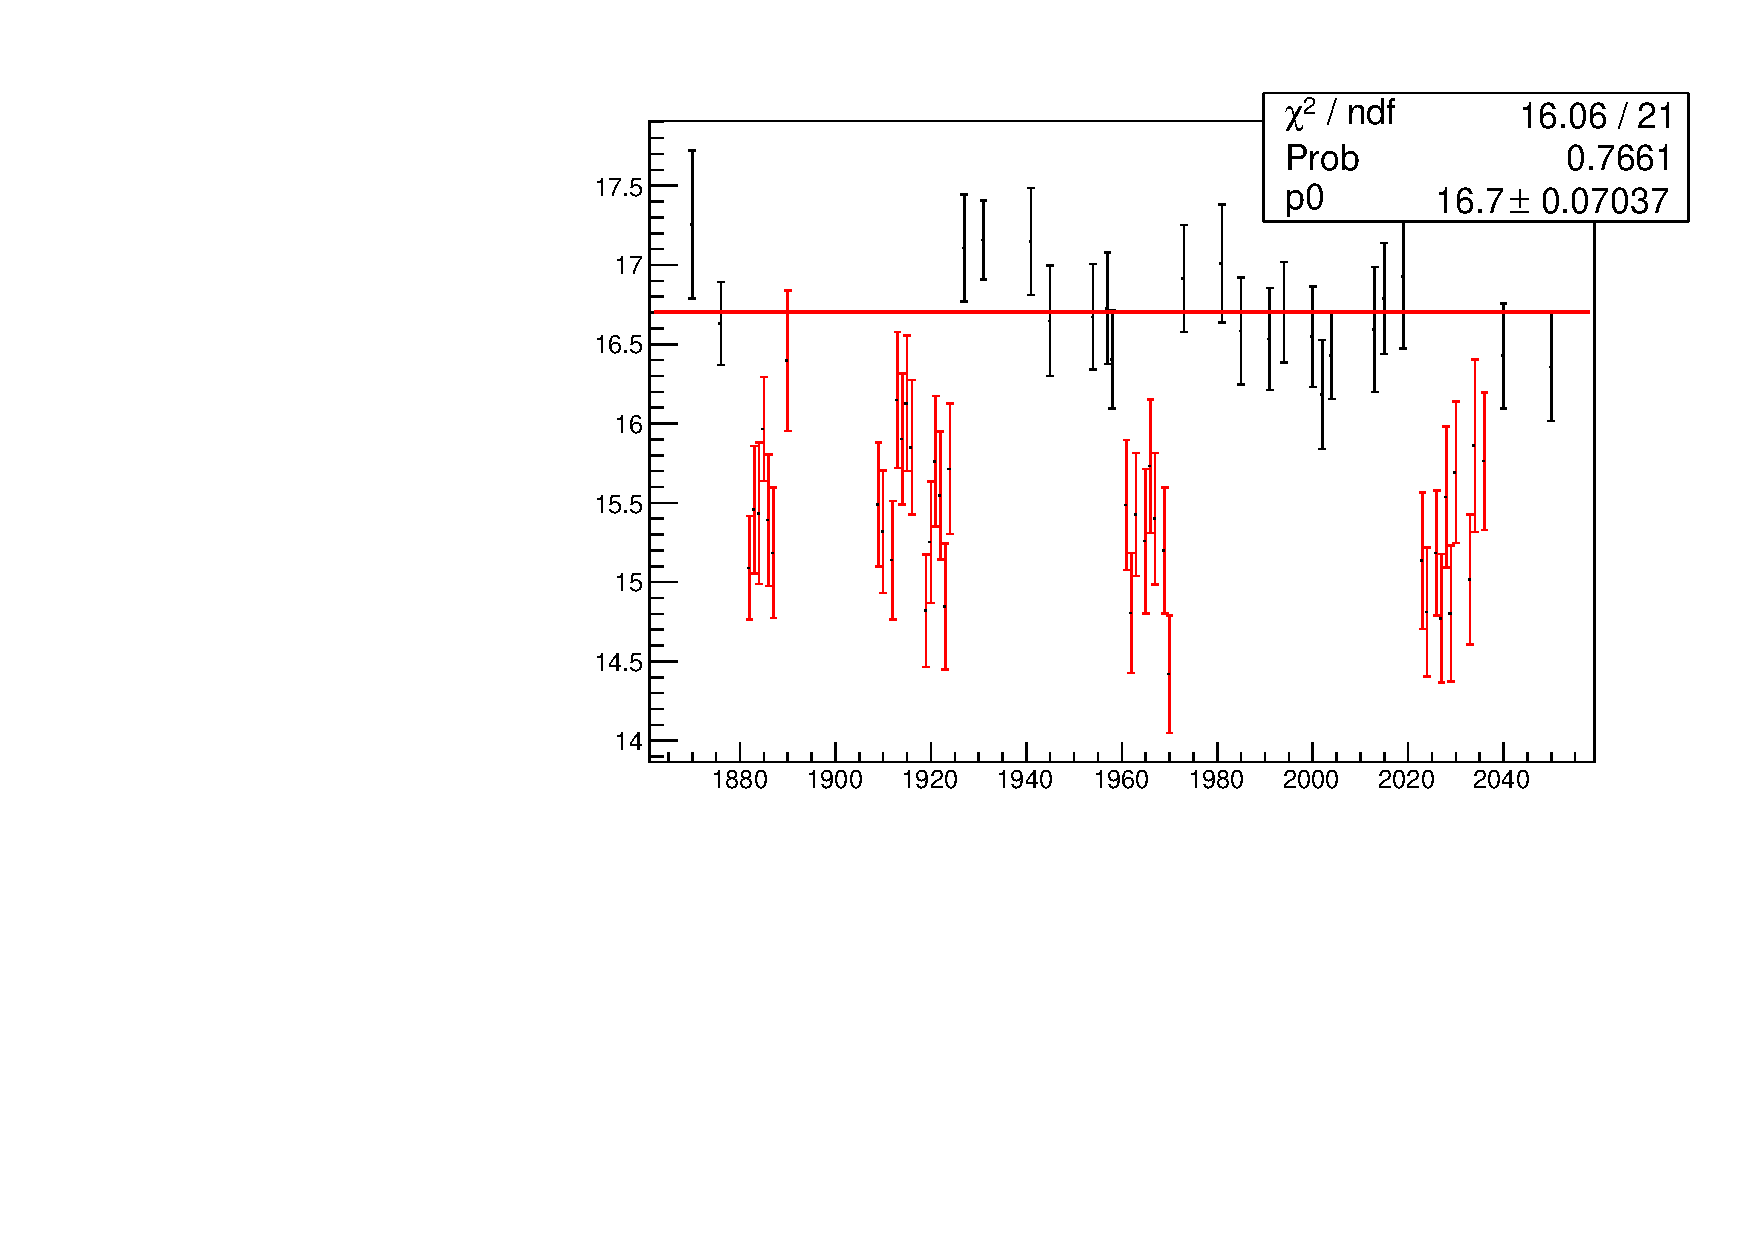
\includegraphics[width=\textwidth]{../transmission_with_prestorage/prestoragelifetime.pdf}
\caption{Storage lifetime in the pre-storage volume determined during all transmission measurements. The black data points are from measurements with a pre-storage time of \SI{15}{\second}, the red from DREx measurements with a pre-storage time of \SI{10}{\second}.}
\label{fig:prestoragelifetime}
\end{figure}

The transmission measurement with normalization during pre-storage is dependent on the storage lifetime in the pre-storage volume. The rate in the He3 detector, which is proportional to the number of UCN in the pre-storage volume, exponentially drops over time, see~fig.~\ref{fig:he3rate}. And the total number detected is
\begin{equation}
N_p^\mathrm{He3} = \int_0^{t_p} N_0 \exp \frac{-t}{\tau_p} dt = N_0 \tau_p \left( 1 - \exp \frac{-t_p}{\tau_p} \right).
\end{equation}
The number detected in the Li6 detector is the number of UCN in the pre-storage volume at the end of the pre-storage period, multiplied with the transmission $T_\mathrm{corr}$:
\begin{equation}
N_c^\mathrm{Li6} = T_\mathrm{corr} N_0 \exp \frac{-t_p}{\tau_p}.
\end{equation}
Hence the Li6-to-He3 ratio is actually a measure of the transmission T modified with a factor dependent on $\tau_p$:
\begin{equation}
\frac{N_c^\mathrm{Li6}}{N_p^\mathrm{He3}} = T_\mathrm{corr} \frac{\exp \frac{-t_p}{\tau_p}}{\tau_p \left( 1 - \exp \frac{-t_p}{\tau_p} \right)}
\end{equation}
This factor can be divided out by measuring the storage lifetime in the pre-storage volume by fitting an exponential decay to the falling He3 rate. However, the resulting transmission uncertainties are significantly increased.

Over time, the storage lifetime in the pre-storage volume determined this way during all standard transmission experiments with a pre-storage time of \SI{15}{\second} fluctuated between \SIlist{16.2;17.2}{\second}, see fig.~\ref{fig:prestoragelifetime}.


\subsection{Results}

\begin{sidewaystable}
\centering
\caption{Results of transmission experiments. If not otherwise noted, all transmission measurements were performed with the listed guides between IV2 and IV3 with their O-rings pointing towards each other and a 90$^\circ$ elbow downstream of IV3. The $\chi^2$ gives an indication of how well the data fits the assumption that the ratios $R$ stay constant over all cycles in each experiment.}
\begin{tabular}{l r r r r r r l}
\toprule
Experiment & Run & $\bar{R}_p$ & $\chi^2/\nu$ & $\bar{R}_\mathrm{corr}$ & $\bar{R}_c$ & $\chi^2/\nu$ & Description \\
\midrule
TCN19-020 & 1876 & $1.999 \pm 0.007$ & 1.28 & $48.7 \pm 0.8$ & $8.315 \pm 0.030$ & 0.61 & UGD19+17, no IV3 \\
TCN19-010 & 1870, 1871 & $1.825 \pm 0.011$ & 1.05 & $43.6 \pm 1.2$ & $7.571 \pm 0.026$ & 0.64 & UGD19+22 (NiP) \\
TCN19-240 & 1927 & $1.890 \pm 0.008$ & 1.16 & $45.4 \pm 0.9$ & $7.792 \pm 0.028$ & 1.47 & UGD02+22 (SS) \\
TCN19-250 & 1931, 1937 & $1.768 \pm 0.006$ & 1.01 & $42.4 \pm 0.6$ & $7.365 \pm 0.019$ & 1.21 & UGD02+19+22 (SS+NiP) \\
TCN19-260 & 1941 & $1.879 \pm 0.009$ & 1.42 & $45.0 \pm 0.9$ & $8.045 \pm 0.29$ & 0.58 & UGD22 \\
TCN19-280v1 & 1945 & $1.848 \pm 0.009$ & 0.91 & $45.0 \pm 1.0$ & $7.533 \pm 0.027$ & 0.77 & vent spider \\
TCN19-280v2 & 1954 & $1.820 \pm 0.008$ & 1.47 & $44.3 \pm 0.9$ & $7.719 \pm 0.028$ & 0.98 & vent spider with plunger full in \\
TCN19-280v3 & 1957 & $1.878 \pm 0.009$ & 0.94 & $45.6 \pm 1.0$ & -- & -- & vent spider with plunger cycled \\
TCN19-280v4 & 1958 & $1.835 \pm 0.008$ & 0.73 & $45.0 \pm 0.9$ & -- & -- & vent spider with plunger full in \\
TCN19-010D & 1973 & $1.810 \pm 0.008$ & 0.50 & $43.7 \pm 0.9$ & $7.584 \pm 0.027$ & 1.02 & UGD19+22 (NiP) \\
TCN19-270 & 1981 & $1.408 \pm 0.007$ & 1.16 & $33.9 \pm 0.8$ & $4.679 \pm 0.017$ & 2.12 & UGD13+14+15+22 (Cu) \\
TCN19-120 & 1985 & $1.804 \pm 0.008$ & 0.99 & $44.0 \pm 0.9$ & $7.203 \pm 0.026$ & 0.75 & UGD37+22 (95mm Al-NiP) \\
\midrule
\multicolumn{8}{l}{Measurements after detector was exposed to light:} \\ 
TCN19-121 & 1991 & $1.522 \pm 0.007$ & 1.39 & $37.2 \pm 0.8$ & -- & -- & UGD36+22 (95mm Al-NiP rough) \\
TCN19-123 & 1994 & $1.645 \pm 0.008$ & 0.71 & $40.0 \pm 0.8$ & $6.655 \pm 0.026$ & 0.94 & UGD39+22 (95mm Al-NiP) \\
TCN19-100 & 2000 & $1.729 \pm 0.008$ & 1.99 & $42.2 \pm 0.9$ & -- & -- & UGD31+33+22 (95mm SS-NiP) \\
TCN19-101 & 2002 & $1.536 \pm 0.007$ & 0.85 & $37.9 \pm 0.8$ & -- & -- & UGD30+32+22 (95mm SS-black NiP) \\
TCN19-120A & 2004, 2005 & $1.650 \pm 0.007$ & 1.35 & $40.4 \pm 0.7$ & $6.615 \pm 0.025$ & 1.35 & UGD37+22 (95mm Al-NiP) \\
TCN19-102 & 2013 & $1.670 \pm 0.008$ & 0.81 & $40.73 \pm 0.9$ & -- & -- & UGD34+35+22 (95mm Al-NiP) \\
TCN19-124 & 2015 & $1.680 \pm 0.008$ & 1.77 & $40.7 \pm 0.9$ & -- & -- & UGD40+22 (95mm SS-NiP smooth) \\
TCN19-010E & 2019 & $1.730 \pm 0.008$ & 1.80 & $41.7 \pm 1.1$ & $7.162 \pm 0.027$ & 0.58 & UGD19+22 (NiP) \\
TCN19-120B & 2040 & $1.631 \pm 0.008$ & 1.66 & $40.0 \pm 0.8$ & -- & -- & UGD37+22 (95mm Al-NiP) \\
TCN19-010B & 2050 & $1.683 \pm 0.009$ & 0.75 & $41.3 \pm 0.9$ & -- & -- & UGD19+22 (NiP) \\
\bottomrule
\end{tabular}
\label{tab:transmission}
\end{sidewaystable}

\begin{sidewaystable}
\centering
\caption{Comparison of transmission experiments.}
\begin{tabular}{l r r r r r}
\toprule
Experiment & Reference & $T_p$ & $T_\mathrm{corr}$ & $T_c$ & Description \\
\midrule
TCN19-010 & TCN19-020 & $0.913 \pm 0.007$ & $0.896 \pm 0.029$ & $0.911 \pm 0.005$ & Transmission of IV3 \\
TCN19-010 & TCN19-260 & $0.972 \pm 0.008$ & $0.969 \pm 0.034$ & $0.941 \pm 0.005$ & Adding UGD19 \\
TCN19-240 & TCN19-260 & $1.006 \pm 0.007$ & $1.007 \pm 0.029$ & $0.969 \pm 0.006$ & Adding UGD02 \\
TCN19-250 & TCN19-260 & $0.941 \pm 0.006$ & $0.941 \pm 0.024$ & $0.915 \pm 0.004$ & Adding UGD02+19 \\
TCN19-270 & TCN19-260 & $0.749 \pm 0.006$ & $0.752 \pm 0.023$ & $0.582 \pm 0.004$ & Adding UGD13+14+15 \\
TCN19-280v1 & TCN19-260 & $0.983 \pm 0.007$ & $0.998 \pm 0.029$ & $0.936 \pm 0.005$ & Spider compared to UGD22 \\
TCN19-280v2 & TCN19-260 & $0.968 \pm 0.008$ & $0.982 \pm 0.028$ & $0.960 \pm 0.005$ & Spider compared to UGD22 \\
TCN19-280v3 & TCN19-260 & $0.999 \pm 0.007$ & $0.984 \pm 0.029$ & -- & Spider compared to UGD22 \\
TCN19-280v4 & TCN19-260 & $0.977 \pm 0.007$ & $1.012 \pm 0.030$ & -- & Spider compared to UGD22 \\
TCN19-120 & TCN19-260 & $0.960 \pm 0.007$ & $0.977 \pm 0.028$ & $0.895 \pm 0.005$ & Adding UGD37 \\
\midrule
\multicolumn{6}{l}{Reproducibility measurements:} \\ 
TCN19-010D & TCN19-010 & $0.992 \pm 0.008$ & $1.002 \pm 0.034$ & $0.998 \pm 0.005$ & Before detector exposure \\
TCN19-010E & TCN19-010 & $0.948 \pm 0.009$ & $0.957 \pm 0.037$ & $0.946 \pm 0.005$ & After and before exposure \\
TCN19-120A & TCN19-120 & $0.914 \pm 0.006$ & $0.919 \pm 0.025$ & $0.918 \pm 0.005$ & After and before exposure \\
TCN19-010B & TCN19-010E & $0.973 \pm 0.008$ & $0.991 \pm 0.034$ & -- & After and before isopure refill \\
TCN19-120B & TCN19-120A & $0.989 \pm 0.008$ & $0.989 \pm 0.027$ & -- & After and before isopure refill \\
\midrule
\multicolumn{5}{l}{Measurements after detector was exposed to light:} \\ 
TCN19-100 & TCN19-120A & $1.048 \pm 0.008$ & $1.044 \pm 0.028$ & -- & SS-NiP compared to Al-NiP \\
TCN19-101 & TCN19-120A & $0.931 \pm 0.006$ & $0.938 \pm 0.026$ & -- & Black NiP compared to Al-NiP \\
TCN19-102 & TCN19-120A & $1.012 \pm 0.007$ & $1.007 \pm 0.030$ & -- & Al-NiP compared to Al-NiP \\
TCN19-121 & TCN19-120A & $0.923 \pm 0.007$ & $0.920 \pm 0.025$ & -- & Rough Al-NiP to Al-NiP \\
TCN19-123 & TCN19-120A & $0.997 \pm 0.007$ & $0.988 \pm 0.026$ & $1.006 \pm 0.006$ & Al-NiP compared to Al-NiP \\
TCN19-124 & TCN19-120A & $1.018 \pm 0.008$ & $1.007 \pm 0.028$ & -- & Smooth SS-NiP to Al-NiP \\
\bottomrule
\end{tabular}
\label{tab:transmission_comparison}
\end{sidewaystable}

Table \ref{tab:transmission} lists the results of the individual transmission experiments and table \ref{tab:transmission_comparison} compares several.



\section{Storage lifetime in the source}
\label{sec:storagelifetime}

To measure the storage lifetime of UCN in the source, we performed several cycles with three periods each. During the first period, the target is irradiated to accumulate UCN in the source with IV1 closed. During the second period, the beam is turned off and the UCN are stored with IV1 closed. In the third period, the valve is opened and the UCN stored in the source are emptied into the detector(s). This cycle is repeated several times with varying duration of the storage period. This measurement was repeated regularly to determine the change of storage lifetime over time.

To determine the storage lifetime, we subtracted the average background rates determined during the storage period, see equation~\ref{eq:transmission_begin}, from the events in the respective detector, and divided it by the average beam current $\bar{I}$ during irradiation:
\begin{equation}
n_c = \frac{N_c}{\bar{I}}.
\end{equation}
To take into account fluctuations of the beam current, its standard deviation during irradiation $\Delta I$ is included in the uncertainty
\begin{equation}
\Delta n_c = n_c \sqrt{ \left( \frac{\Delta N_c}{N_c} \right)^2 + \left( \frac{\Delta I}{\bar{I}} \right)^2 }.
\end{equation}

\begin{figure}
\centering
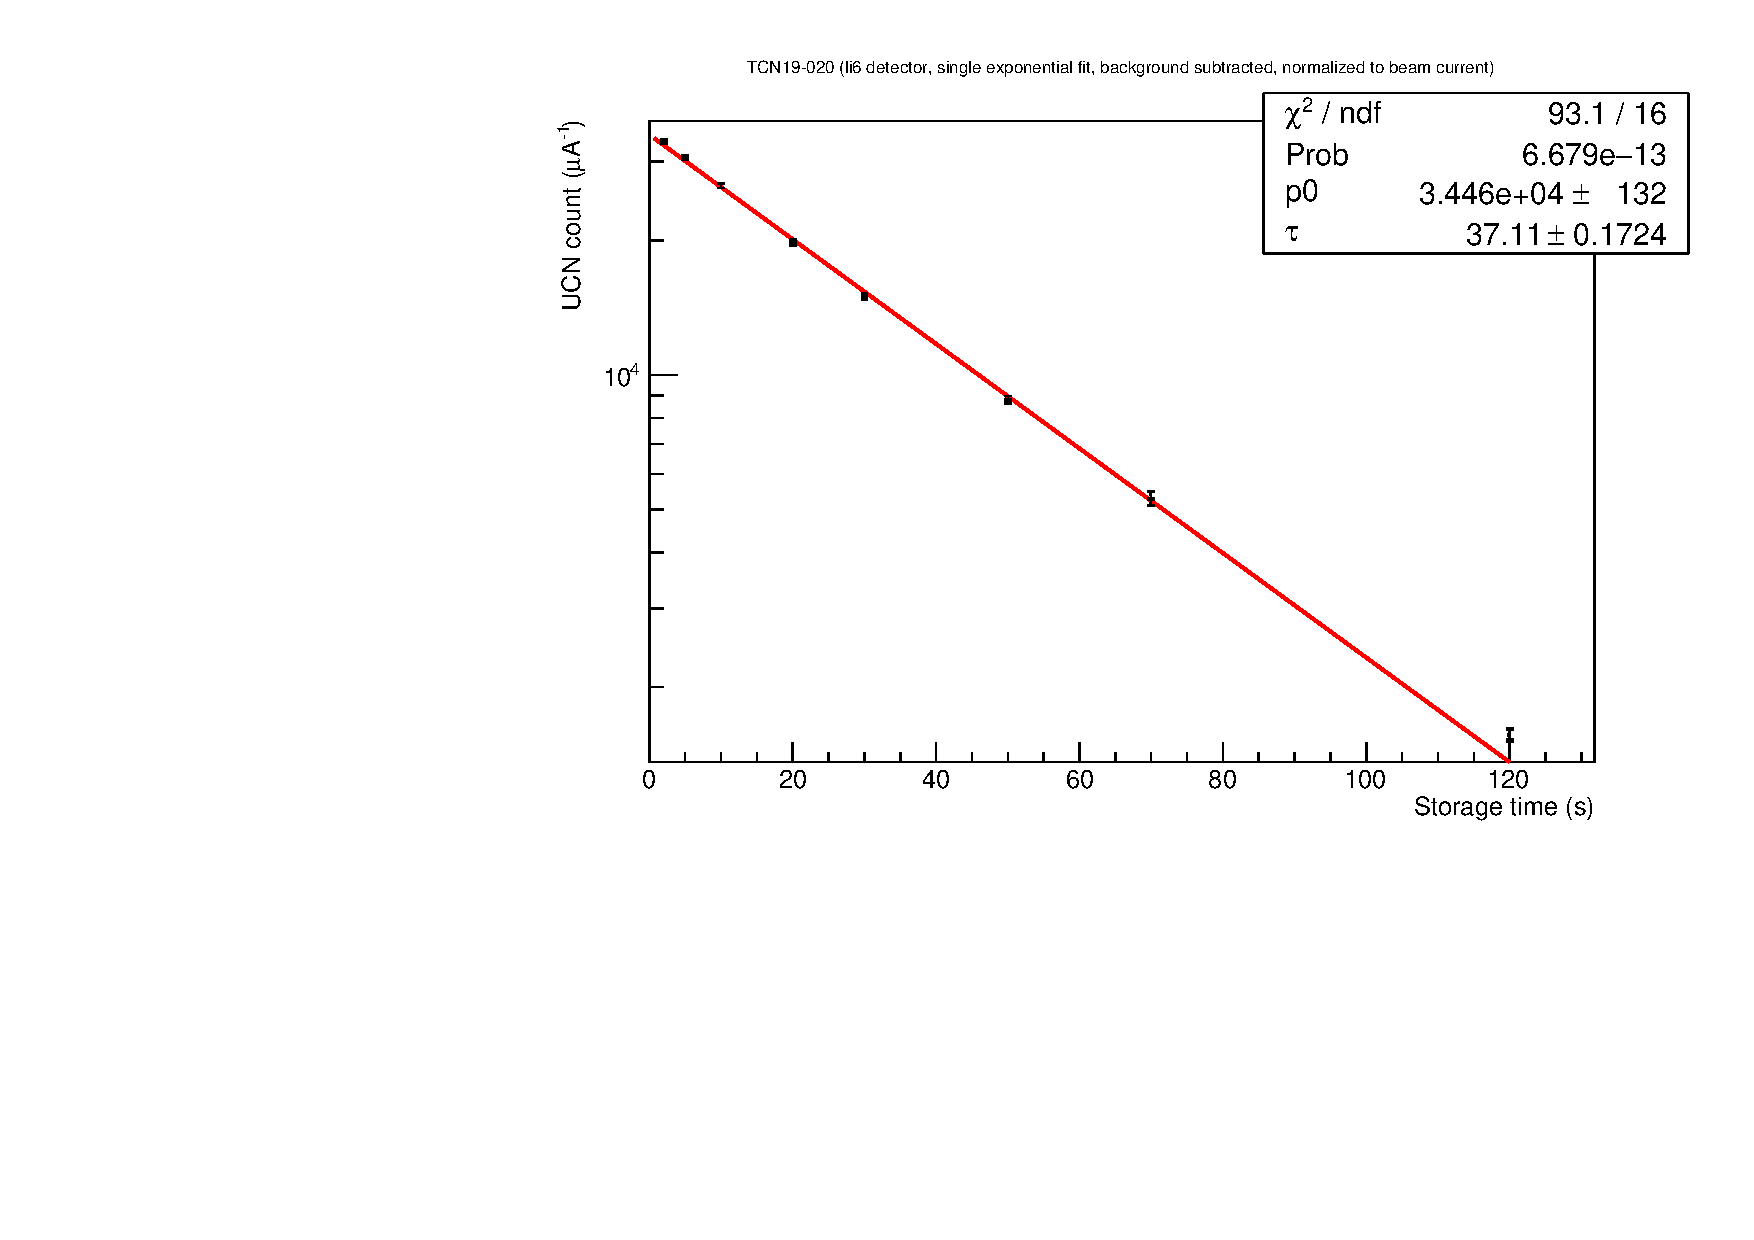
\includegraphics[width=\textwidth,page=1]{../storagelifetime/TCN19-020_1873.pdf}
\includegraphics[width=\textwidth,page=2]{../storagelifetime/TCN19-020_1873.pdf}
\caption{Number of UCN detected in the Li6 detector (top) and the He3 detector (bottom) divided by average beam current, after different storage times during one of the regular storage-lifetime experiments (TCN18-015, run 1019). A single exponential fit determines the storage lifetime.}
\label{fig:storagelifetime}
\end{figure}

Ideally, the number of detected UCN should drop exponentially with increasing storage time and the exponential time constant is the storage lifetime, see fig.~\ref{fig:storagelifetime}. Compared to 2018, however, the source seemed to operate more stably with smaller changes of liquid-helium temperatures and smaller fluctuations of the UCN yield.



\subsection{Excluded cycles}

Individual cycles are excluded from the analyzed storage-lifetime data if
\begin{itemize}
\item no beam data was available (2 cycles);
\item the beam current dropped below \SI{0.1}{\micro\ampere} (7 cycles);
\item the beam current fluctuated by more than \SI{0.02}{\micro\ampere} (1 cycle);
\item the last period does not contain any Li6 events, i.e. the run was aborted at some point during this cycle (11 cycles);
\item IV1 never opened (6 cycles); or
\item no events were detected during the irradiation period (1 cycle).
\end{itemize}

In total, 28 out of 351 cycles had to be excluded.

\subsection{Change of storage lifetime over time}

\begin{figure}
\centering
\includegraphics[width=\textwidth,page=2]{../storagelifetime/dailytau.pdf}
\caption{Storage lifetimes on different dates determined from an exponential fit to the UCN counts in the Li6 detector (black) and the He3 detector (red) during the regular storage-lifetime measurements. The grey areas indicate when the production volume was refilled with isopure helium.}
\label{fig:dailytau}
\end{figure}

\begin{figure}
\centering
\includegraphics[width=\textwidth,page=2]{../storagelifetime/tauvstemp.pdf}
\caption{Correlation of storage lifetimes with vapor pressure, measured with the Li6 detector. The two measurements at the bottom left were performed after the isopure-helium refill.}
\label{fig:tauvstemp}
\end{figure}

The storage lifetime in the source seemed to gradually decrease over time, see fig.~\ref{fig:dailytau}, and slightly recover after the UCN-production volume was refilled with isopure helium. Part of this change was correlated to a gradual increase in vapor pressure and temperature of the isopure helium, see fig.~\ref{fig:tauvstemp}, presumably caused by the gradually dropping helium level in the production volume.


\section{Storage lifetime in guide components}

To determine the storage lifetime in different guide components we ran experiments with three periods per cycle. An irradiation period, where UCN are produced and filled into the component, with the valve IV3 to the detector closed. A storage period, where the irradiation is stopped and all the UCN valves are closed. And a counting period, where the valve to the detector is opened to count the UCN remaining in the component. The He3 detector again serves as monitor detector, measuring the UCN density and storage lifetime in the volume between IV1 and IV2.

\begin{figure}
\centering
\includegraphics[width=\textwidth,page=6]{{"../storagelifetime_with_monitor/TCN19-240 (UGD02+22)"}.pdf}
\caption{Rate in the He3 detector during a measurement of storage lifetime in a guide component. The rate detected after the irradiation is a measure of the UCN density filled into the guide component. An exponential fit determines the storage lifetime between IV1 and IV2.}
\label{fig:He3rate_storage}
\end{figure}

UCN remaining in the component after storage are counted with the Li6 detector. The average background determined during the storage period is subtracted using equations (\ref{eq:transmission_begin})--(\ref{eq:background_subtraction_end}) and then normalized using the counts in the He3 detector after the irradiation ended, see fig.~\ref{fig:He3rate_storage}. The He3 counts are accumulated over the minimal duration of a measurement cycle with \SI{0}{\second} storage time, i.e. the counting time (typically \SI{120}{\second}).

\begin{figure}
\centering
\includegraphics[width=\textwidth,page=3]{{"../storagelifetime_with_monitor/TCN19-240 (UGD02+22)"}.pdf}
\caption{Background-corrected and normalized number of UCN detected in the Li6 detector after different storage times in guides UGD22 and UGD2 between valves IV2 and IV3 (TCN18-081). Cycles with a storage time of \SI{0}{\second} are excluded from the single exponential fit.}
\label{fig:storagelifetime_with_monitor_Li6}
\end{figure}

This is repeated for several different storage times. The background-corrected, normalized number of detected UCN is assumed to drop exponentially with storage time. The storage lifetime $\tau_\mathrm{s}$ is determined with a single exponential fit, see fig.~\ref{fig:storagelifetime_with_monitor_Li6}. We excluded cycles with a storage time of \SI{0}{\second} (i.e. valve to the detector opening at the same time as the valve(s) to the source closing) from the fit, since UCN could simply be transmitted through both still partially open valves and not have been stored at all.

\begin{figure}
\centering
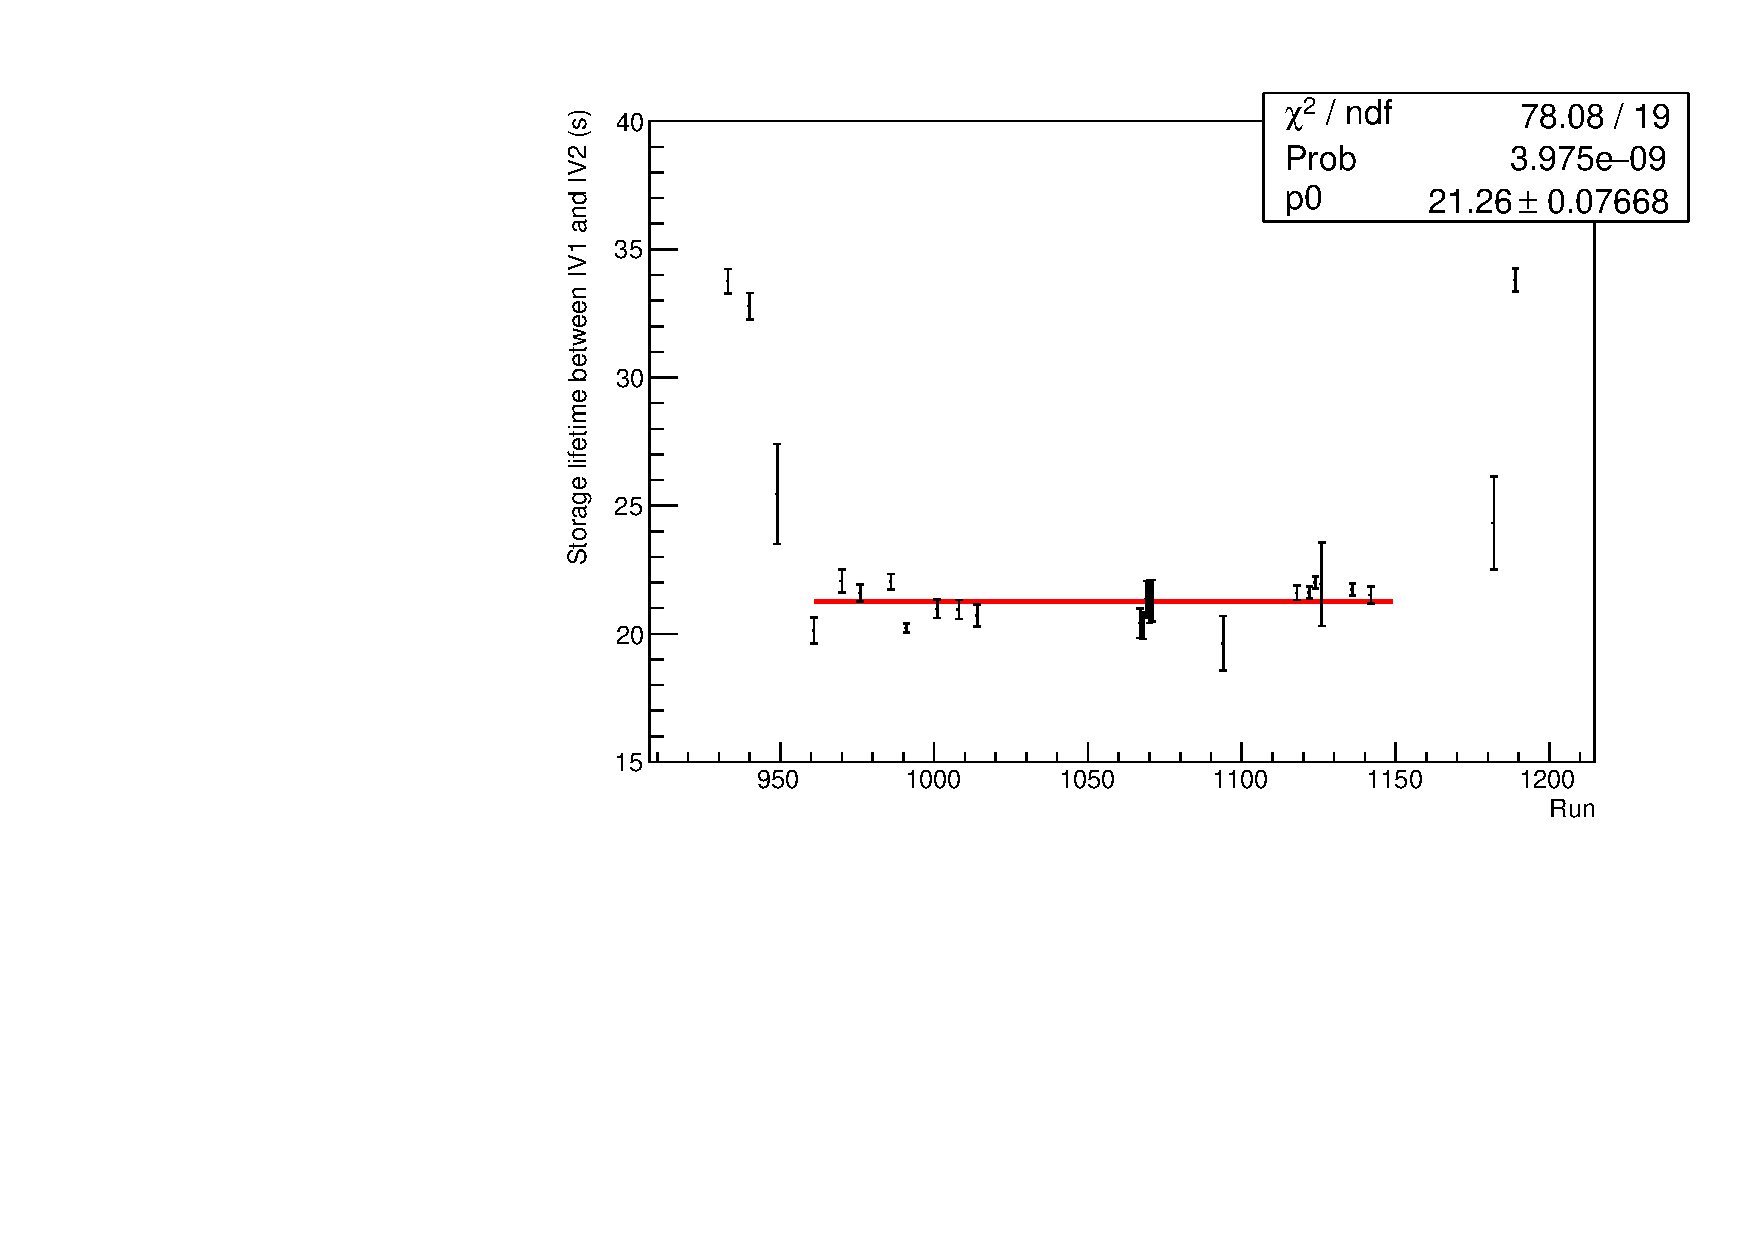
\includegraphics[width=\textwidth]{../storagelifetime_with_monitor/pinhole.pdf}
\caption{Storage lifetime between IV1 and IV2, measured with the pinhole method. The red line shows the average over all runs where this guide section was unchanged. The first three runs where performed with IV2 flipped, giving higher storage lifetimes. The last two runs were performed in the higher position, resulting in a softer UCN spectrum and longer storage lifetimes.}
\label{fig:pinhole}
\end{figure}

An exponential fit to the rate in the He3 rate can also confirm the measurements of storage lifetime between IV1 and IV2 that are used to normalize the transmission measurements. These lifetimes are slightly longer than in the transmission experiments, between \SIlist{18.8;19.8}{\second}, probably due to the longer measurement time, but the overall variation of \SI{1}{\second} is similar, see fig.~\ref{fig:pinhole}.

\subsection{Excluded cycles}

Individual cycles are excluded from the analyzed transmission data if
\begin{itemize}
\item no beam data was available (4 cycles);
\item the beam current dropped below \SI{0.8}{\micro\ampere} (20 cycles);
\item the beam current fluctuated by more than \SI{0.02}{\micro\ampere} (1 cycle);
\item the last period does not contain any Li6 events, i.e. the run was aborted at some point during this cycle (17 cycles);
\item IV1 never opened (0 cycles);
\item the He3 detector detected less than 1000 UCN during irradiation (0 cycles);
\item the Li6 detector detected a large background rate above \SI{10}{\hertz} during the irradiation or background period (3 cycles).
\end{itemize}

In total, 45 out of 456 cycles had to be excluded.

\subsection{Results}

\begin{sidewaystable}
\caption{Results of storage experiments in different guide components. All measurements were performed with the listed guides between IV2 and IV3 with their O-rings pointing towards each other and a \SI{90}{\degree} elbow downstream of IV3. The $\chi^2$ gives an indication of how well the data fits the single exponential. The struck-out entries were affected by large variations of the Li6 background or, in the last row, by instability of the source.}
\begin{tabular}{l r r r l}
\toprule
Experiment & Runs & $\tau_\mathrm{s}$ & $\chi^2/\nu$ & Description \\
\midrule
TCN19-010 & 1847, 1850 & \sout{$34.6 \pm 0.6$} & 4.20 & UGD19+22 \\
TCN19-240 & 1928 & $39.9 \pm 0.4$ & 1.60 & UGD02+22 \\
TCN19-250 & 1934, 1938 & $39.7 \pm 0.3$ & 1.65 & UGD02+19+22 \\
TCN19-260 & 1942 & \sout{$31.4 \pm 0.8$} & 6.57 & UGD22 \\
TCN19-280v1 & 1946 & $20.1 \pm 0.8$ & 0.69 & vent spider \\
TCN19-280v2 & 1951 & $21.3 \pm 0.8$ & 0.67 & vent spider with plunger full in \\
TCN19-280v3 & 1956 & $19.9 \pm 0.7$ & 1.06 & vent spider with pluger cycled \\
TCN19-280v4 & 1959 & $23.2 \pm 0.8$ & 1.14 & vent spider with plunger full in \\
TCN19-010D & 1979, 1980 & $36.8 \pm 0.4$ & 1.13 & UGD19+22 \\
TCN19-270 & 1983 & $19.4 \pm 0.4$ & 0.91 & UGD13+14+15+22 \\
TCN19-120 & 1986 & $53.8 \pm 0.6$ & 2.08 & UGD37+22 (95mm Al-NiP) \\
TCN19-121 & 1992 & $49.8 \pm 0.6$ & 1.40 & UGD36+22 (95mm Al-NiP rough) \\
TCN19-123 & 1996 & $53.1 \pm 0.6$ & 1.57 & UGD39+22 (95mm Al-NiP) \\
TCN19-100 & 2001 & $47.2 \pm 0.6$ & 1.30 & UGD31+33+22 (95mm SS-NiP) \\
TCN19-101 & 2003 & $12.7 \pm 0.3$ & 2.78 & UGD30+32+22 (95mm SS-black NiP) \\
TCN19-120A & 2007 & $52.09 \pm 0.7$ & 0.98 & UGD37+22 (95mm Al-NiP) \\
TCN19-102 & 2014 & $42.7 \pm 0.5$ & 1.56 & UGD34+35+22 (95mm Al-NiP) \\
TCN19-124 & 2016 & $41.8 \pm 0.6$ & 1.09 & UGD40+22 (95mm SS-NiP smooth) \\
TCN19-010E & 2020 & $36.8 \pm 0.6$ & 2.02 & UGD19+22 \\
TCN19-120B & 2041, 2043 & \sout{$50.3 \pm 0.5$} & 147 & UGD37+22 \\
TCN19-010B & 2044, 2045 & \sout{$34.6 \pm 0.6$} & 4.2 & UGD19+22 \\
\bottomrule
\end{tabular}
\label{tab:storagelifetime_with_monitor}
\end{sidewaystable}

The results, see table \ref{tab:storagelifetime_with_monitor}, seem much more stable than in 2018, with almost all fitting nicely to an exponential with a reduced $\chi^2 < 2$. The cases with larger $\chi^2$ can be traced back to large variations in detector background or, in the case of TCN19-010B, to instabilities in the source.

\section{Background rates}
\label{sec:background}

\begin{figure}
\centering
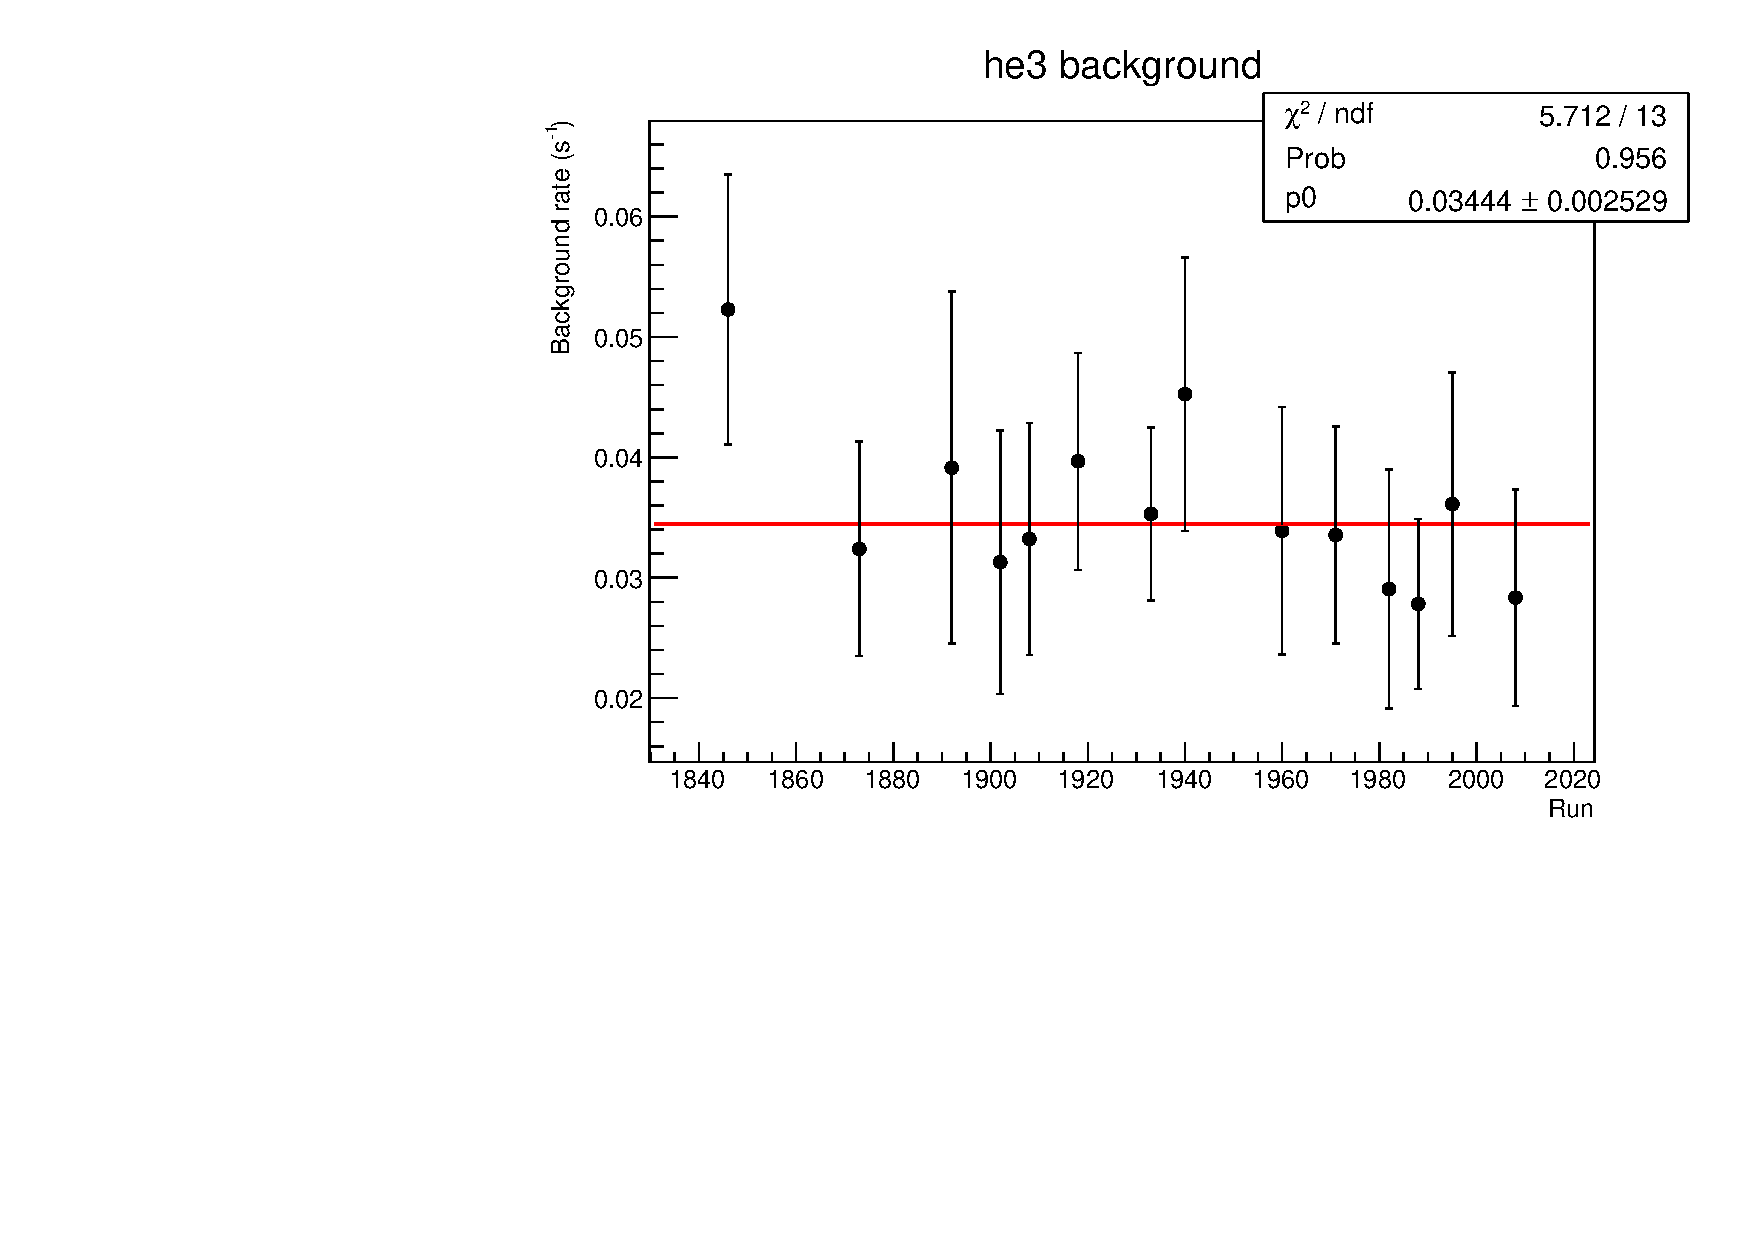
\includegraphics[width=\textwidth]{../storagelifetime/he3_background.pdf}
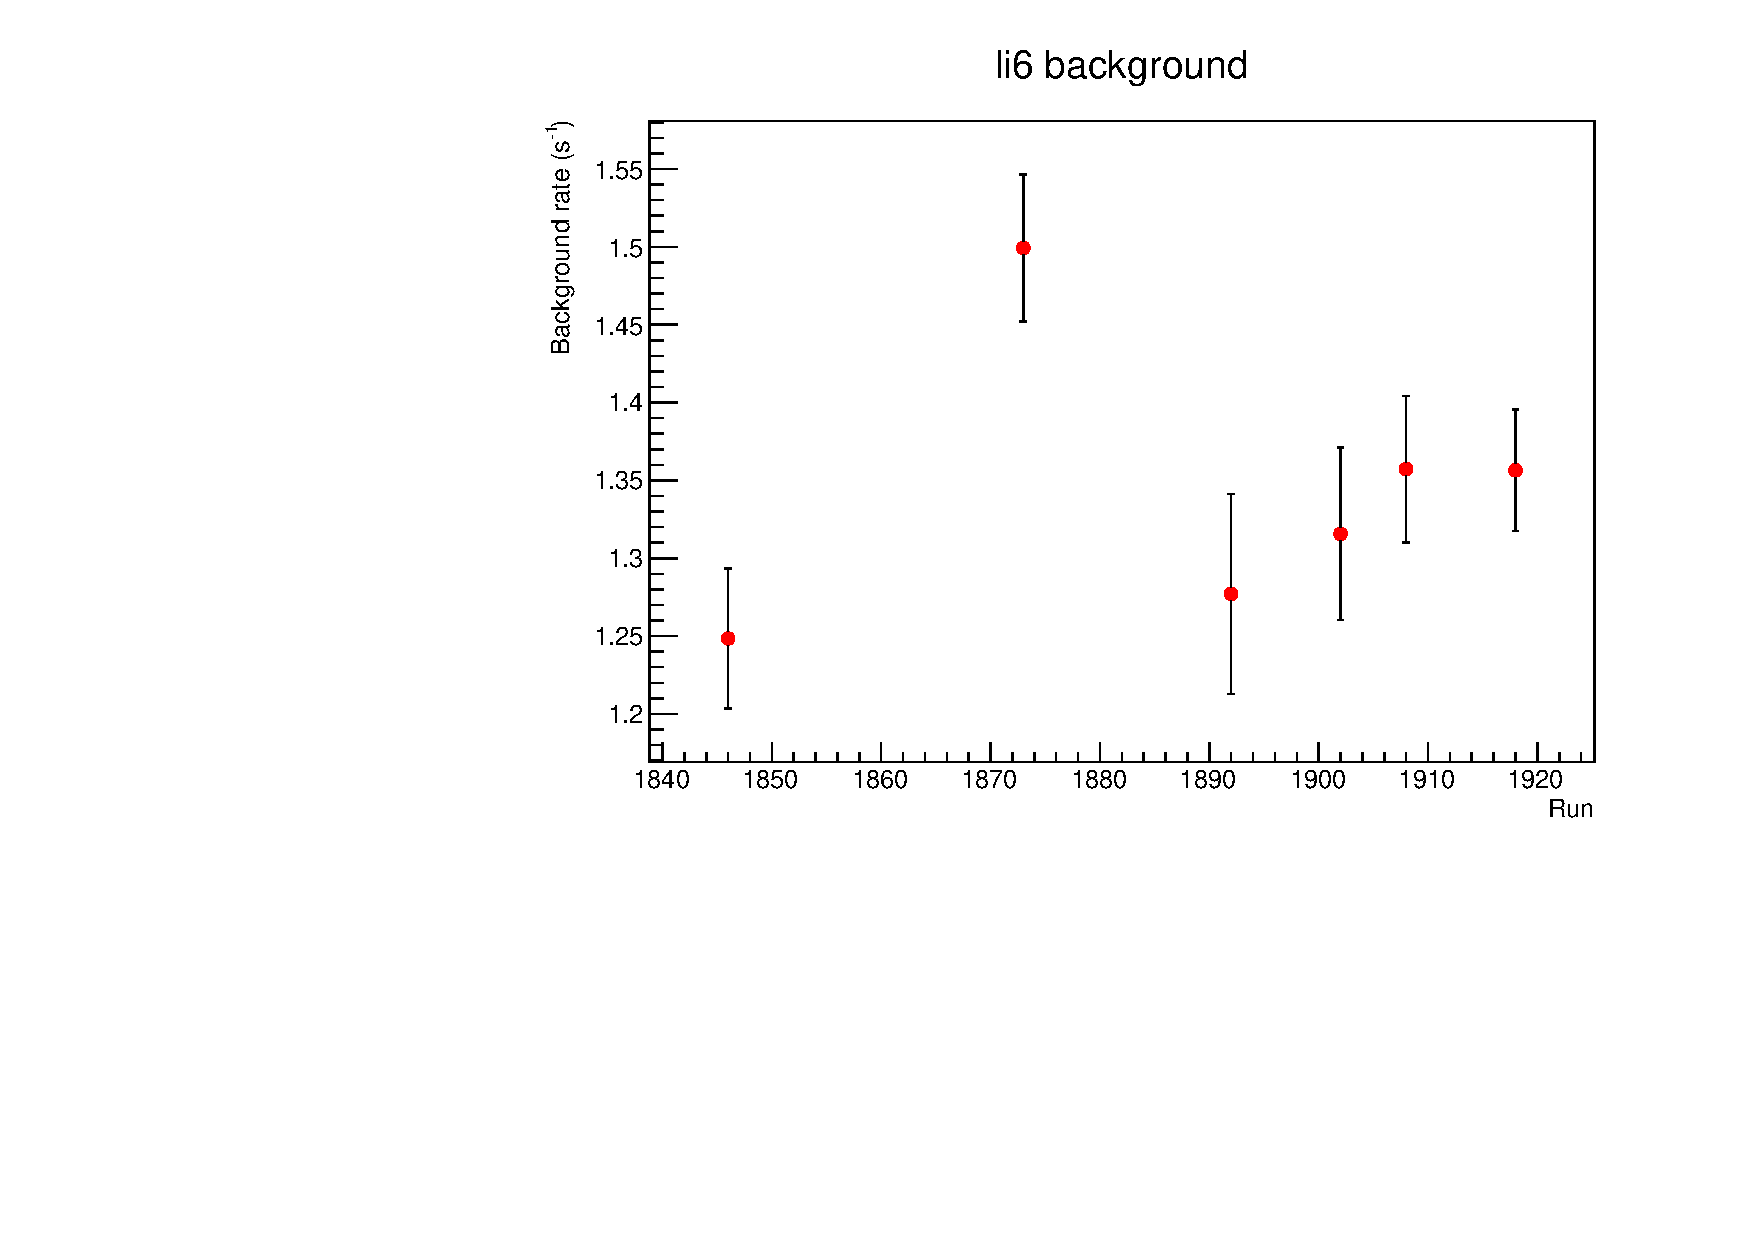
\includegraphics[width=\textwidth]{../storagelifetime/li6_background.pdf}
\caption{Background rates in the He3 (top) and Li6 (bottom) detectors averaged over all storage periods of each measurement of storage lifetime in the source. The red line indicates the overall average. The first three runs, where the Li6 detector was connected to the DAQ but not used for the actual measurement, were excluded from the overall average.}
\label{fig:background1}
\end{figure}

We used the storage periods in the storage-lifetime measurements to estimate background rates of the Li6 and He3 detectors. When measuring storage lifetime in the source, both detectors are separated from the source by vacuum-tight valves, so we assumed that no UCN can leak from the source into the detectors. The background rate in the He3 detector proved to be very stable around an average of \SI{0.0345 +- 0.0022}{\per\second}, see fig.~\ref{fig:background1}. The Li6 detector had a much higher background rate of \SI{1.543 +- 0.012}{\per\second}, slightly lower than in 2018, but still 45 times more than the He3 detector, and showed more fluctuations between measurements. It seemed to be correlated with the beam current in 1A. The first measurement of storage in a guide in fig.~\ref{fig:background2} was performed at a 1A beam current of \SI{38}{\micro\ampere}.

\begin{figure}
\centering
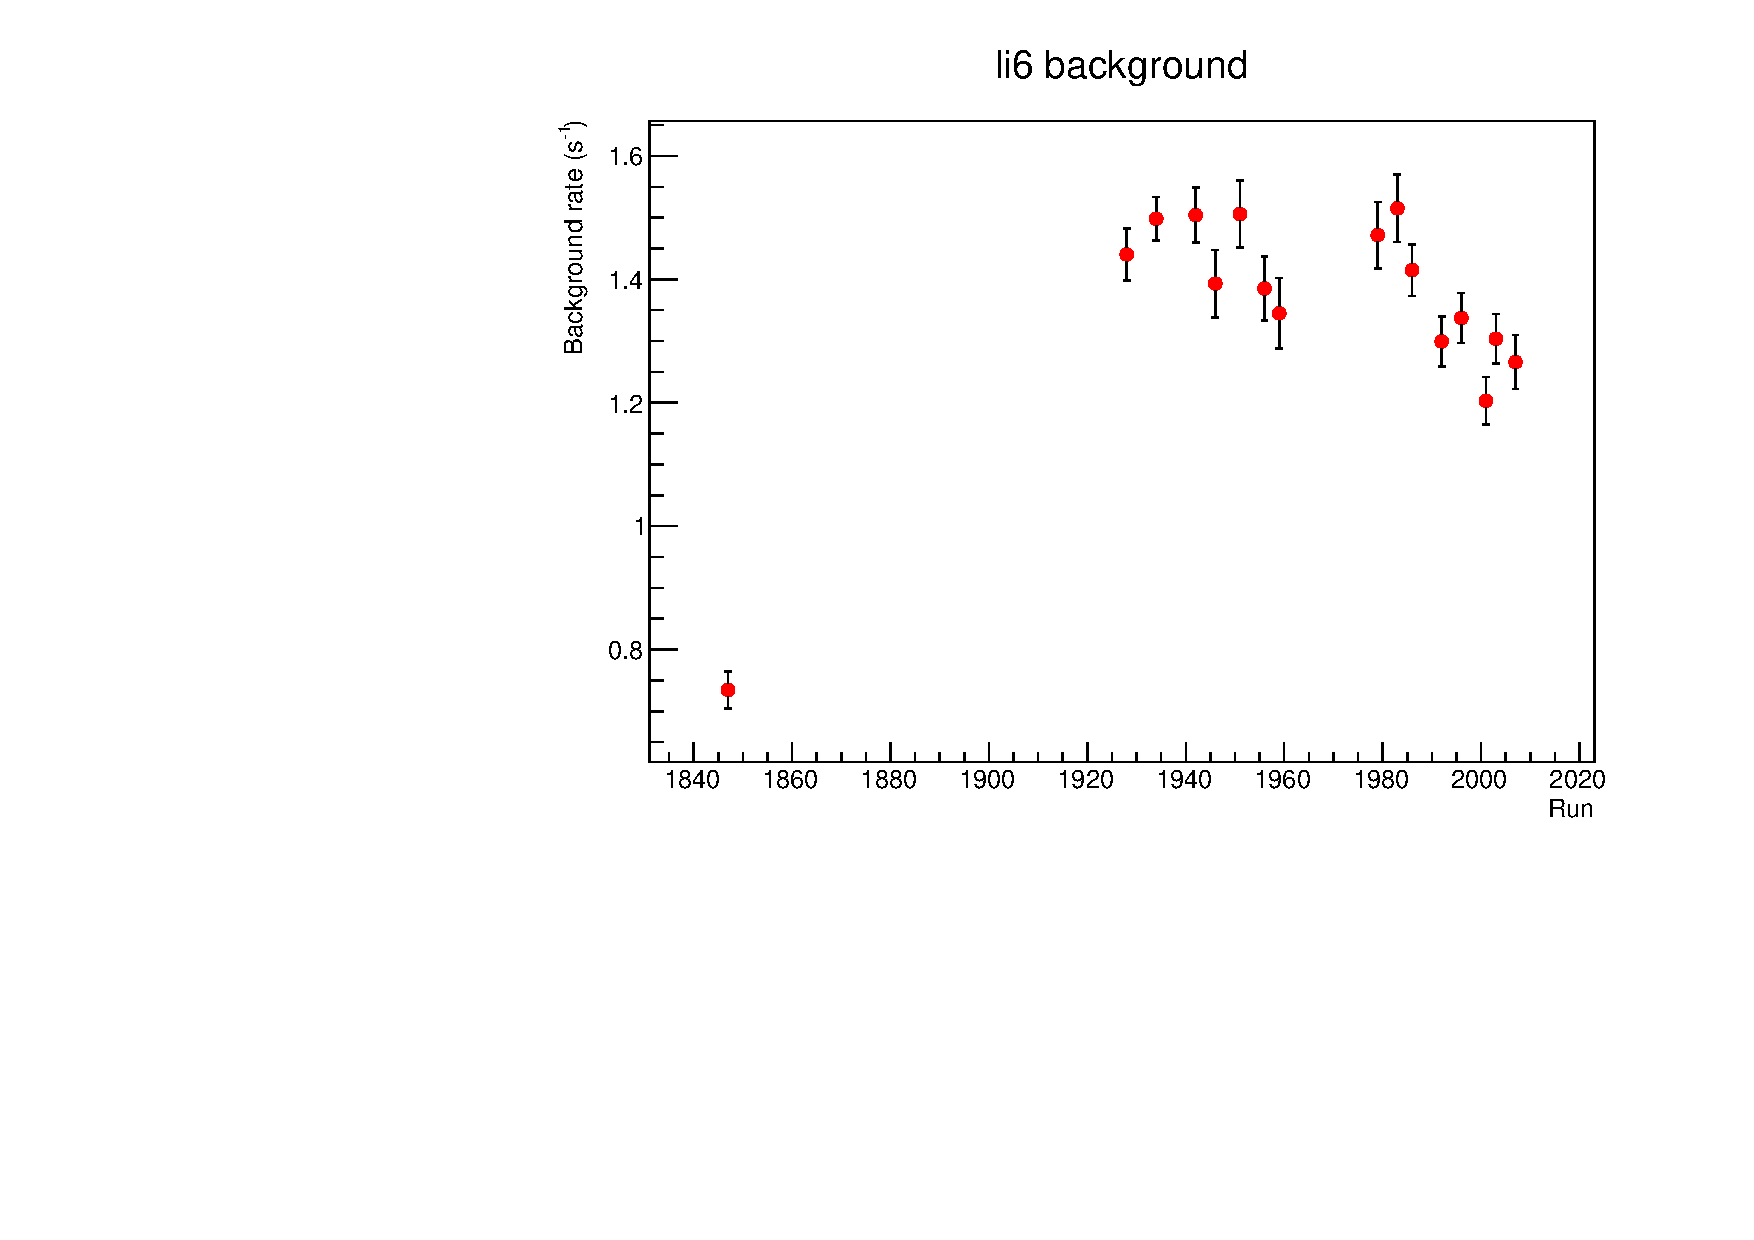
\includegraphics[width=\textwidth]{../storagelifetime_with_monitor/li6_background.pdf}
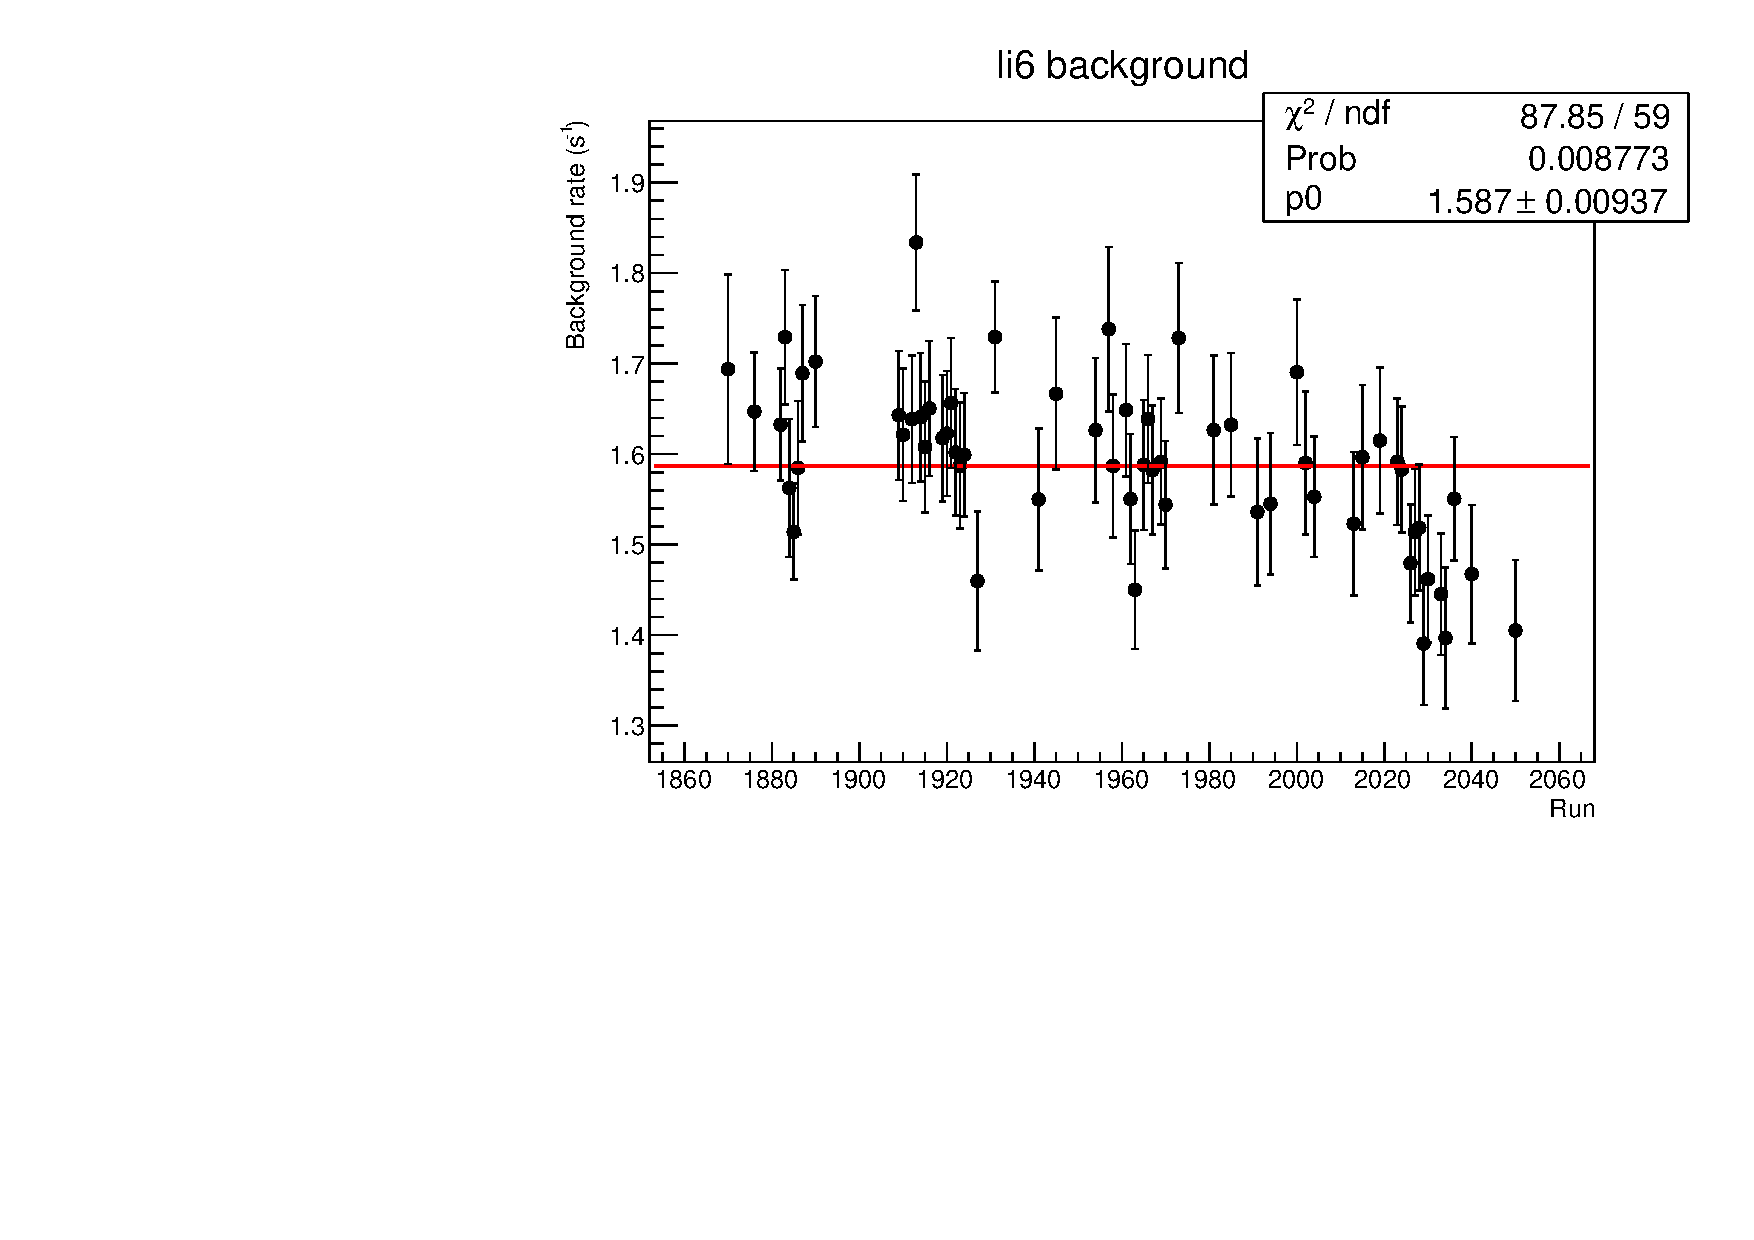
\includegraphics[width=\textwidth]{../transmission_with_prestorage/li6_background.pdf}
\caption{Background rate in the Li6 detector averaged over all storage periods during measurements of storage lifetime (top) or transmission (bottom) of a guide component. The first and last data point in the top graph were taken while beamline 1A operated at lower beam current and are excluded from the average.}
\label{fig:background2}
\end{figure}

\begin{table}
\centering
\caption{Background rates averaged over all cycles of each measurement type.}
\begin{tabular}{l r r r}
\toprule
& & & Additional during \\
Experiment & Detector & Background (\si{\per\second}) & irrad. (\si{\per\second\per\micro\ampere}) \\
\midrule
Storage lifetime & He3 & $0.0345 \pm 0.0022$ & $0.0653 \pm 0.0023$ \\
Storage lifetime & Li6 & $1.543 \pm 0.012$ & $4.264 \pm 0.018$ \\
Storage lifetime guides & Li6 & $1.561 \pm 0.011$ & $4.158 \pm 0.016$ \\
Transm. w/ pre-storage & Li6 & $1.587 \pm 0.009$ & $4.308 \pm 0.007$ \\
Transmission & Li6 & -- & $4.267 \pm 0.019$ \\
\bottomrule
\end{tabular}
\label{tab:backgrounds}
\end{table}

During storage-lifetime measurements in guide components and transmission measurements, the He3 detector is always connected to the source, but the storage periods can be used to determine background in the Li6 detector, see table~\ref{tab:backgrounds}.

While the target was irradiated with protons, both detectors saw a significant increase in background rate. To estimate the increase, we subtracted the previously determined background from the UCN counted during the irradiation period, and normalized the result to beam current. The He3 detector saw an increase in background rate of \SI{190}{\percent} at \SI{1}{\micro\ampere}, the Li6 detector an increase of \SI{280}{\percent}, see table~\ref{tab:backgrounds}.



\end{document}
